\section{Conclusions}

Here we present some conclusions drawn from our visualisations.

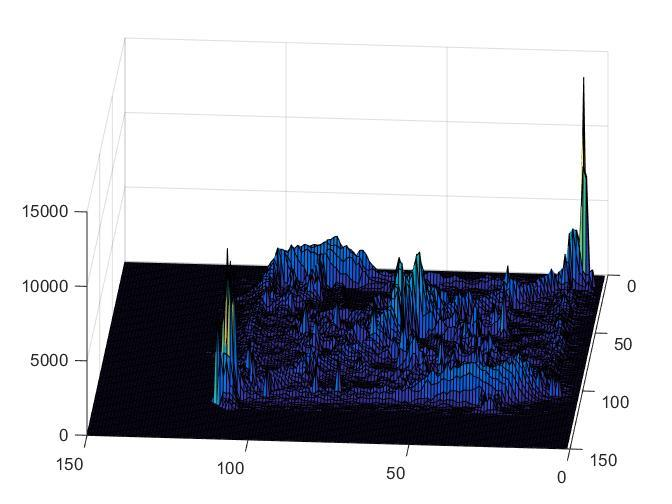
\includegraphics[width=\textwidth]{HM3D}
Here we show a raw, unnormalized 3D heatmap generated in MatLab. It shows two spikes on the starting areas. These might be the player starting positions, but almost look like outliners and might also indicate some errors.

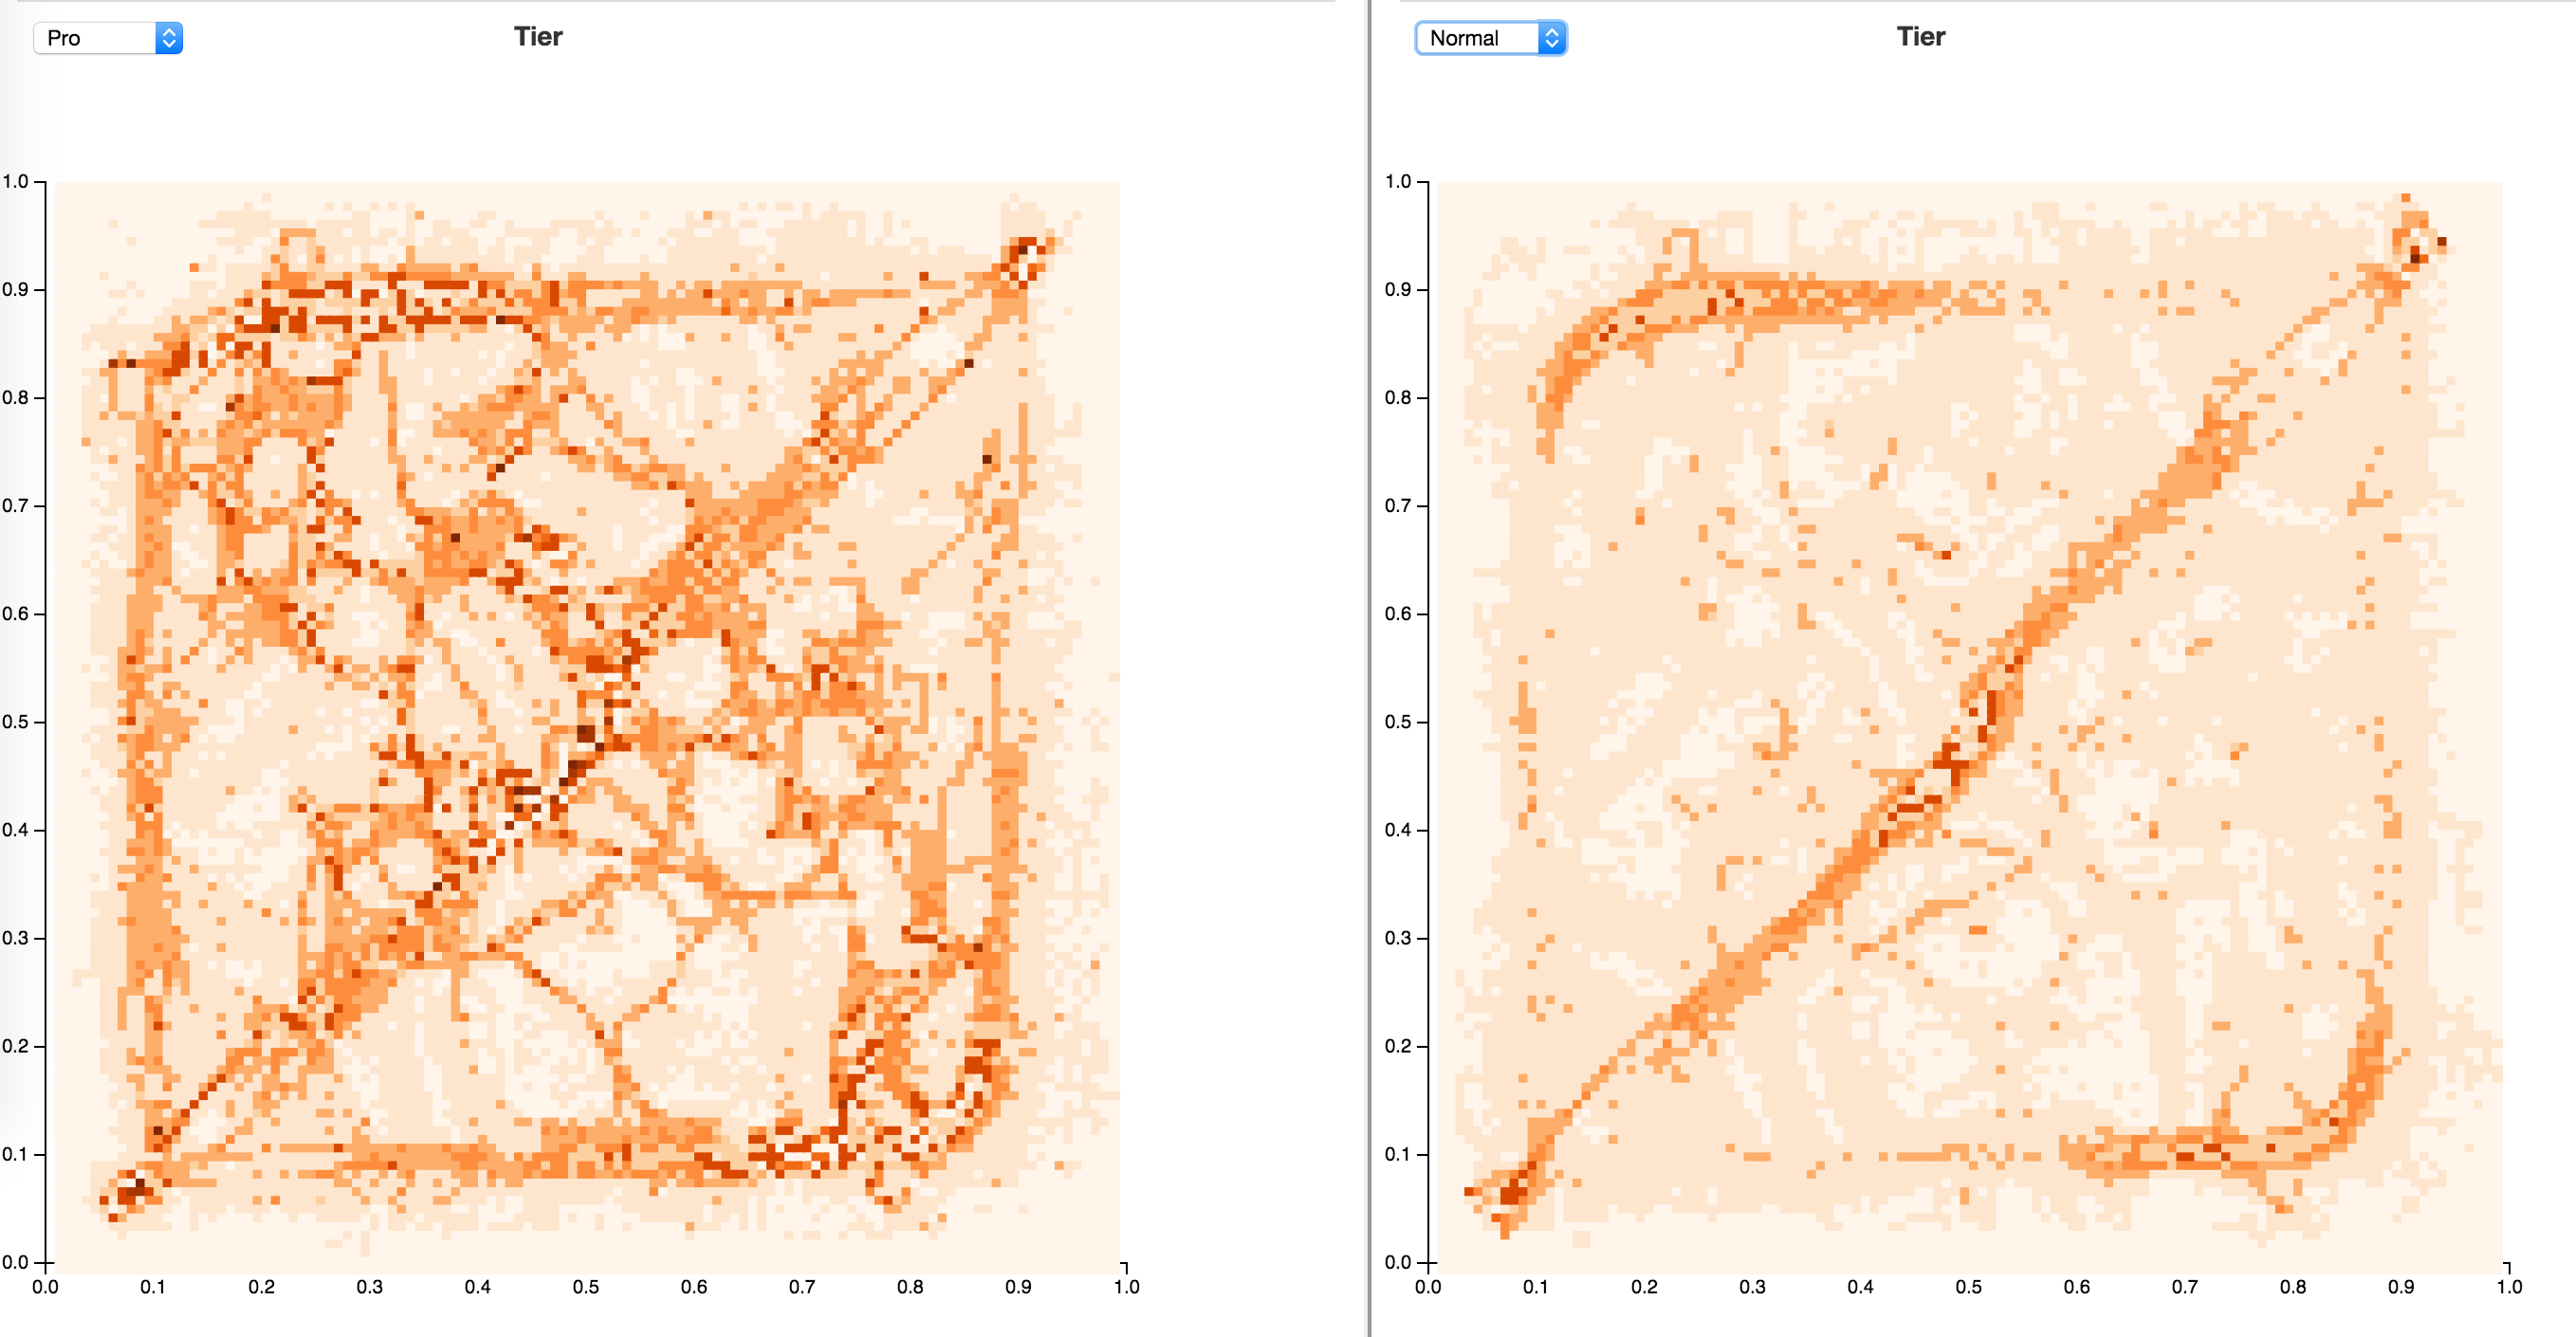
\includegraphics[width=\textwidth]{HM_tiers}

This image compares the heatmaps from a pro tier (left) and normal tier (right). We can clearly see how the normal skill tier mostly fights in lanes and rarely fights in the jungle area, while the pro tier spends a lot more time in the jungle.

Here we see the early game, mid game and end game distributions from one match.

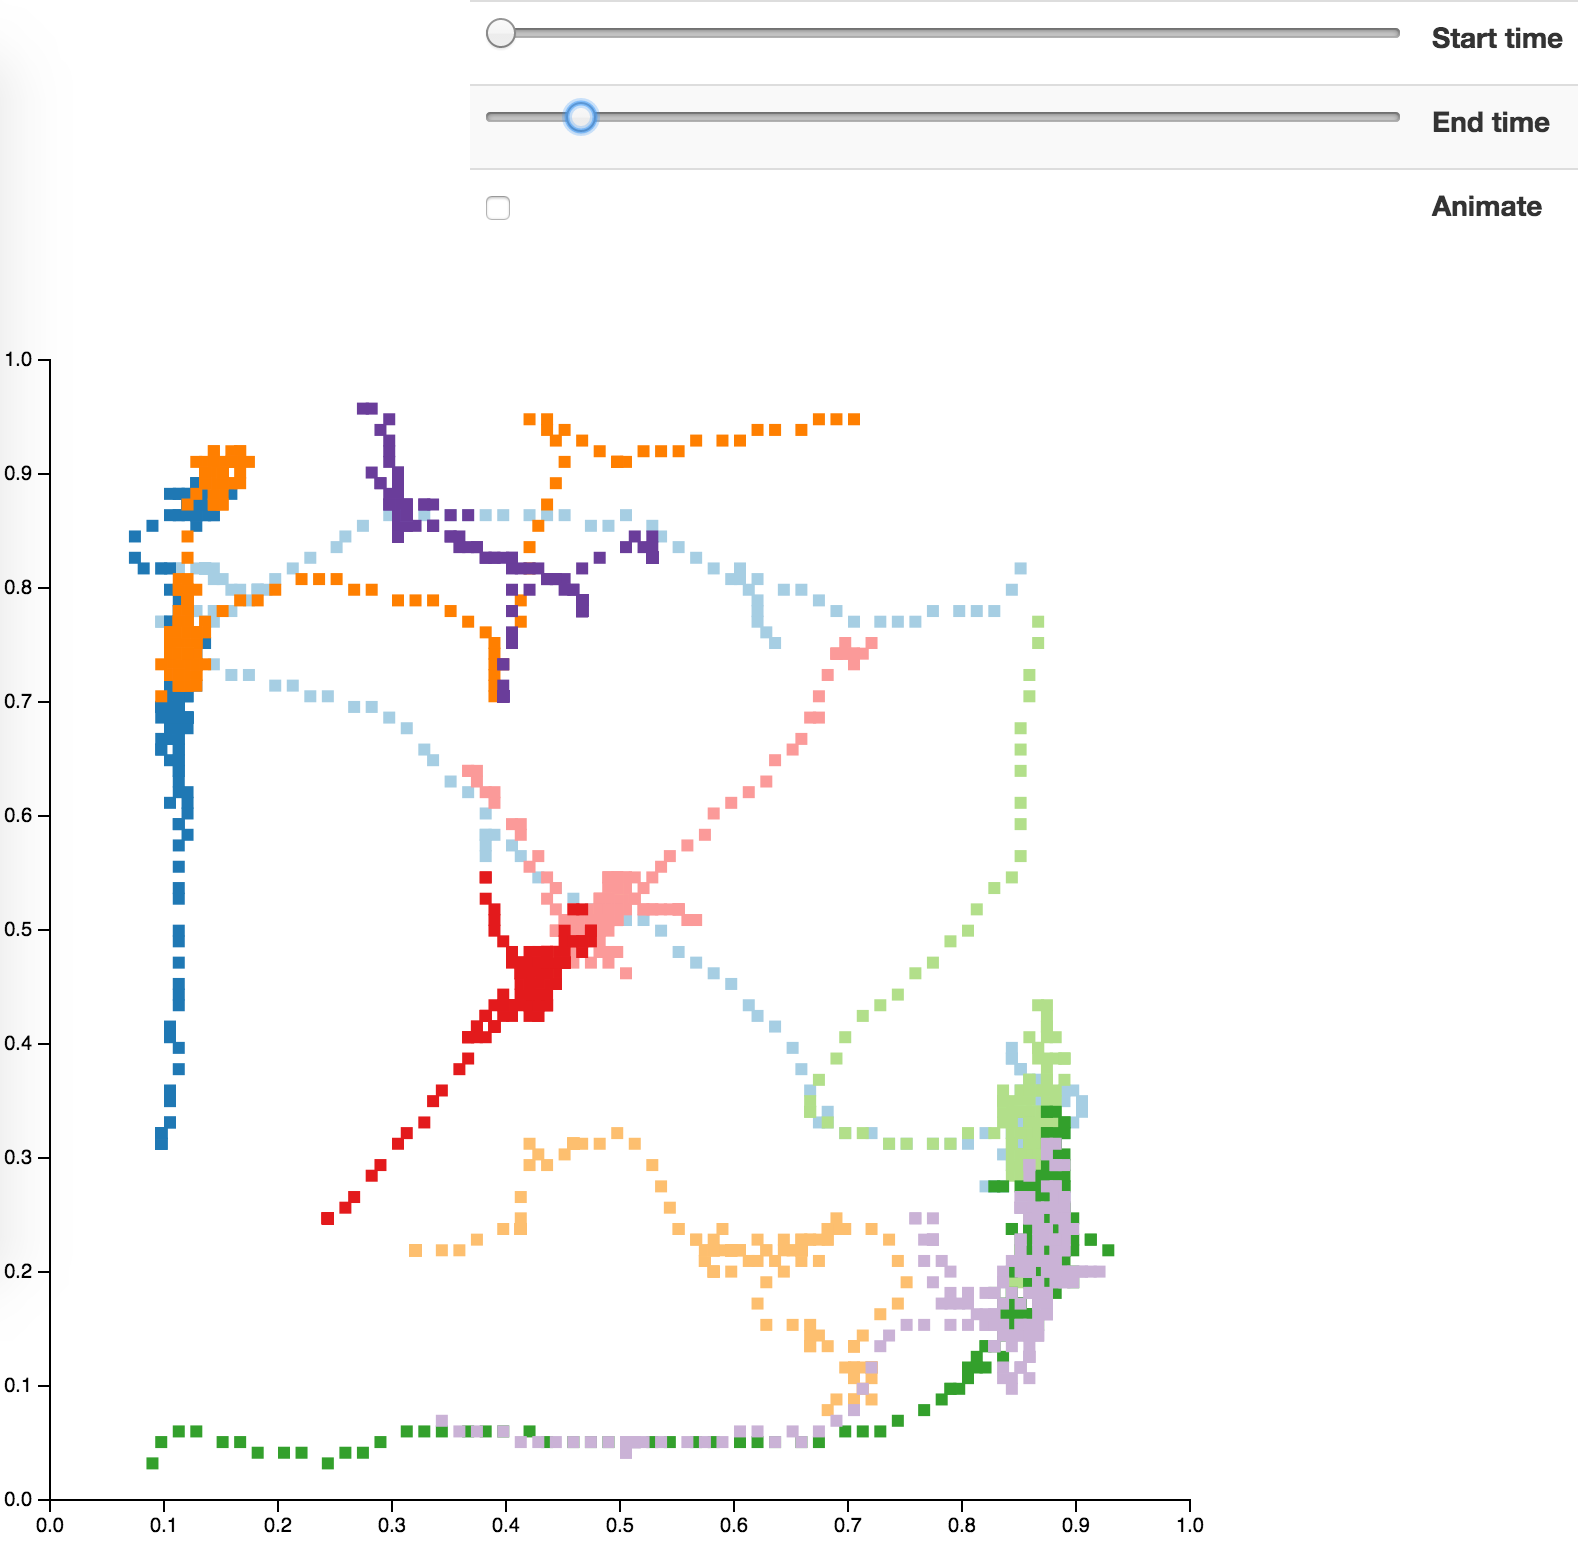
\includegraphics[width=0.7\textwidth]{earlygame}

In the early game we see the players moving into their respective lanes and exchange some blows.

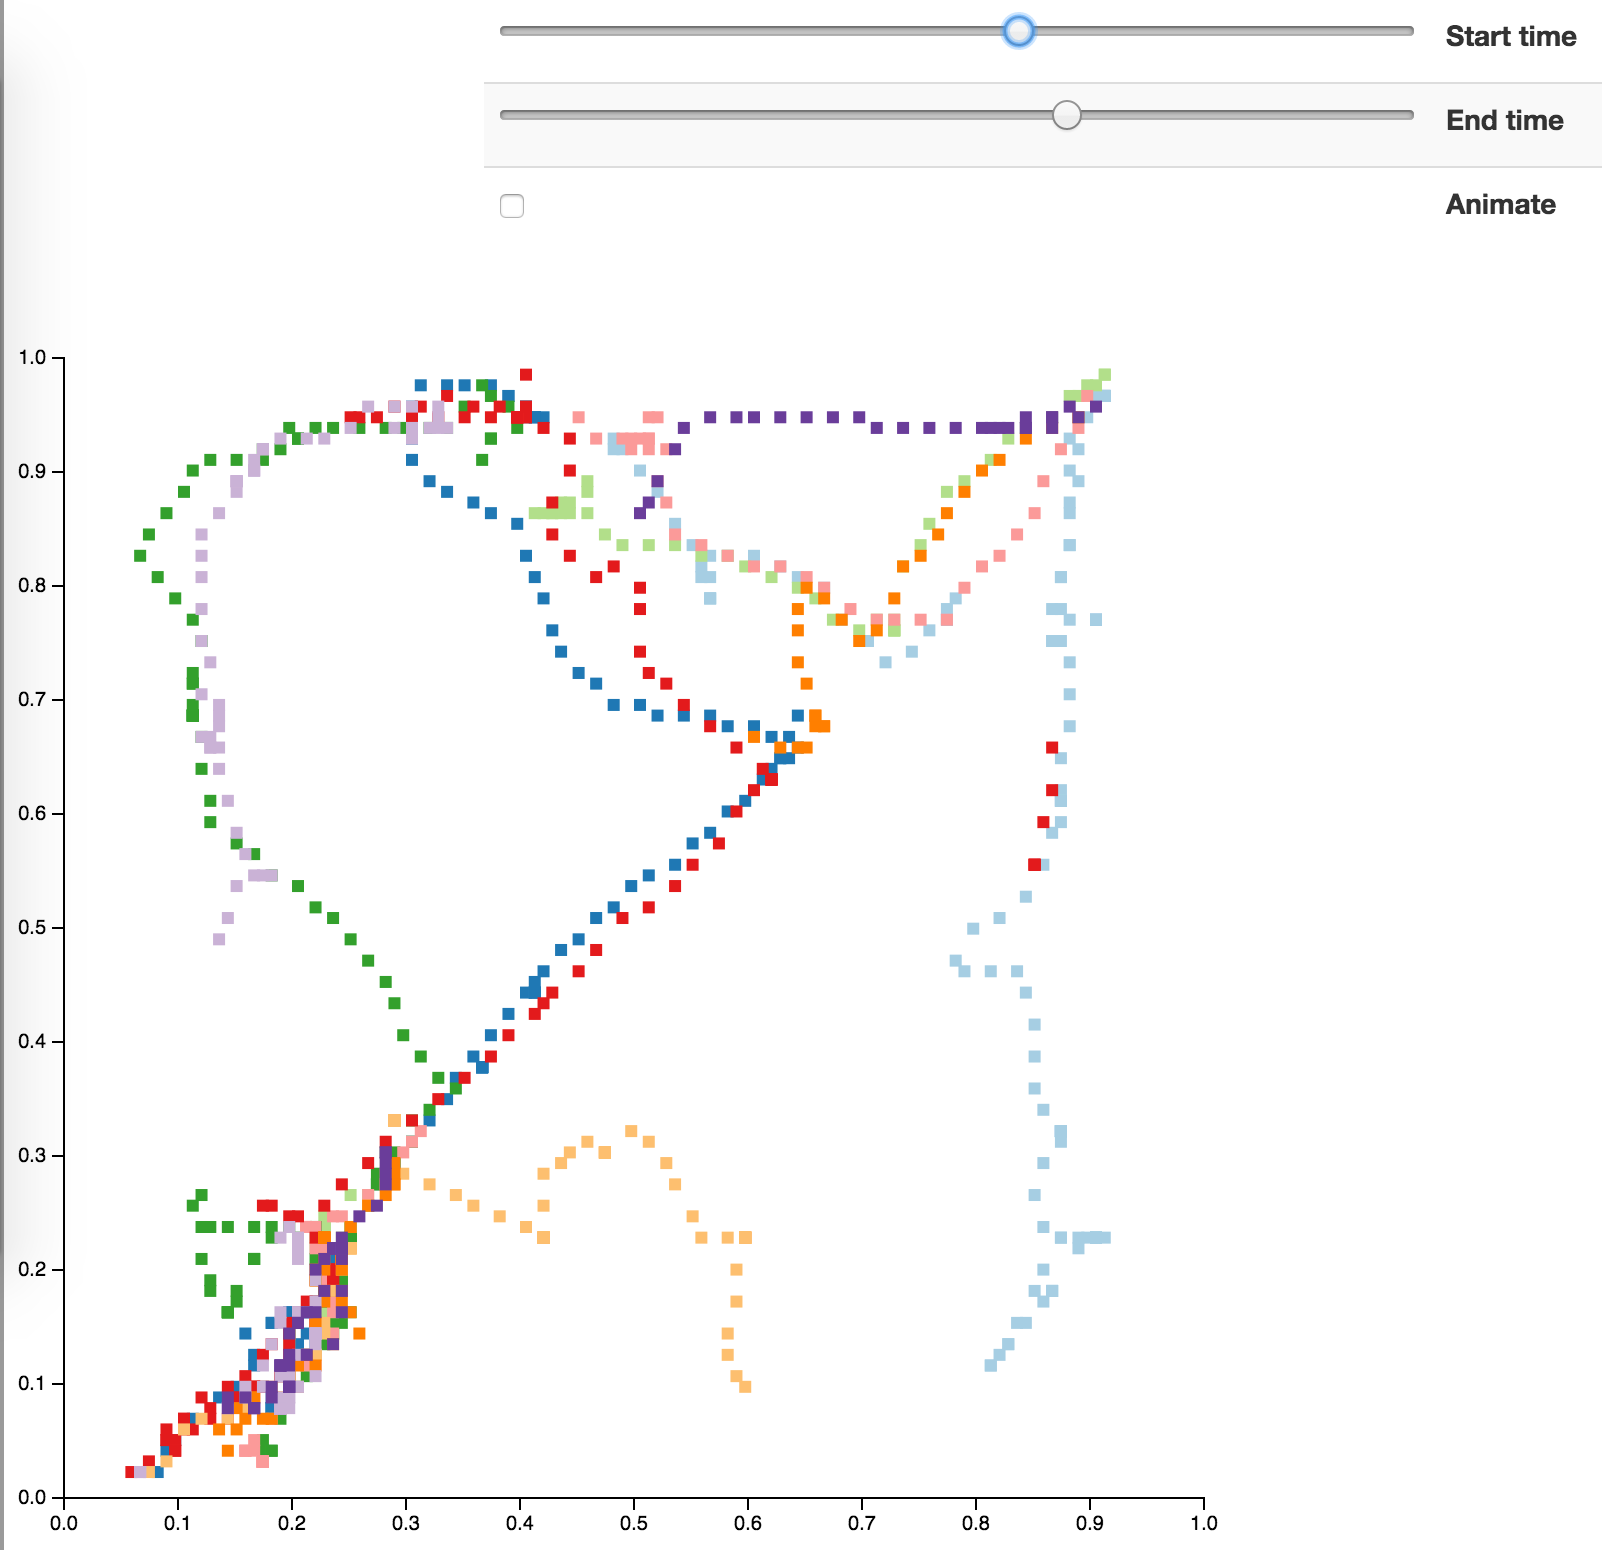
\includegraphics[width=0.7\textwidth]{midgame}

In the late-midgame we see that the game progressed out of their laning phases, and the action is moving towards the bottom team's base. We can see that they most probably lost the middle lane and are behind.

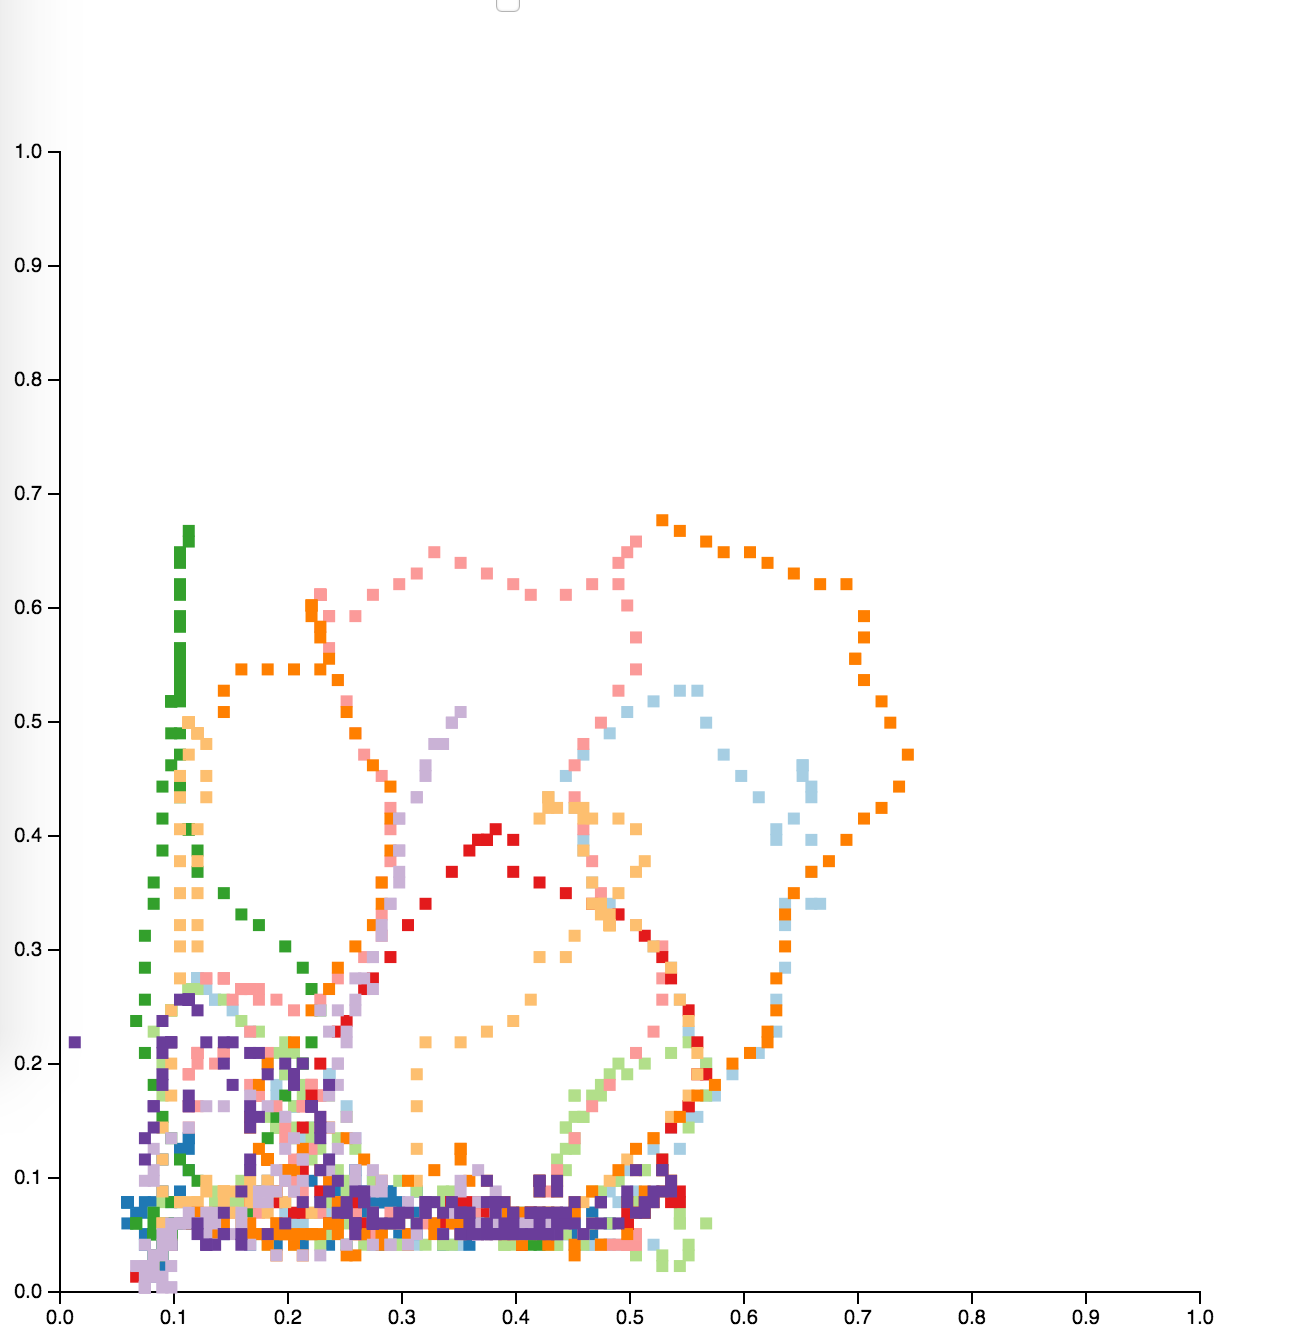
\includegraphics[width=0.7\textwidth]{lategame}

Late game confirms this by exclusively showing heavy fighting in the bottom lane and the bottom team's base. The game ended here, so we can conclude that the top team won.


Another visualization that we thought of doing was to plot the each player's distance from the \textit{radiant's} base for a single match:

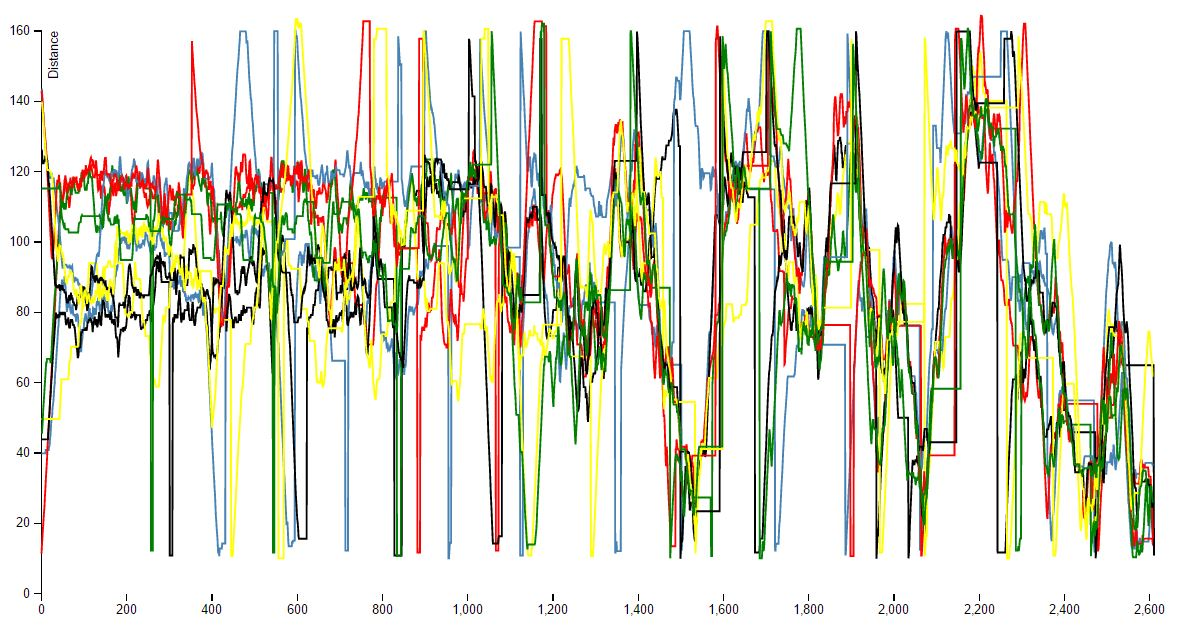
\includegraphics[width=0.9\textwidth]{distance}

From this simple visualization we can see where the majority of the game is played relatively to the base. Every spike that we see on the bottom and the top of the graph is the player either being teleported back to base station or dies and has to start all over. Furthermore we see that there is an interesting pile up towards the end of the game where all the players are concentrated at the radient's base: This is the case where this team is trying to protect their base and the other team is destroying them. We called this a \textit{beta} analysis because we believe that extracting similar information from multiple games ranging from all the different tiers can provide even better insights.

